\section{Data and evaluation protocol}
\label{sec:data}

\subsection{SPX option chains}

The real data are end-of-day SPX option chains from OptionsDX, 16:00\,ET snapshots for 2010--2023
(\spxDays{} trading days). For each expiry the forward $F$ and discount factor $D$ are estimated
from put--call parity, $C-P=D(F-K)$, by regressing $C-P$ on $K$ over the strikes nearest the money
(\cref{app:forwards}), so no rate or dividend data are needed. Implied volatilities are re-inverted
with Black's formula~\citep{black1976} from bid, ask and mid of out-of-the-money options. The model
coordinates are $k=\log(K/F)$, $T$ in years (ACT/365), and total implied variance
$w(k,T)=\sigma^2(k,T)\,T$. A quote is kept if it has $7\le$ DTE $\le 730$, a positive bid below the
ask, a relative spread $(a-b)/m\le 1$, $k\in[-1.5,0.75]$ and $k/(\sigma_{\text{ATM}}\sqrt{T})\in[-6,4]$,
in an expiry with at least eight such quotes. Quotes that are legs of a vertical or butterfly
arbitrage at bid and ask are flagged model-free; they are scored but never fitted.

The chains change a great deal over the sample (\cref{fig:data}). A typical day has about
\spxFirstYearQuotes{} quotes in 12--13 expiries in 2010, 2{,}400 in about 30 expiries in 2016--2017
and \spxValQuotes{} in 37 in 2022, and median half-spreads fall from about 0.75\vp{} to 0.14--0.20\vp{}
and 0.10\vp{} (0.07\vp{} in 2023). Because flags are measured in half-spreads, a fixed margin is a
larger deviation in vol points in the older windows.

\begin{figure}[t]
  \centering
  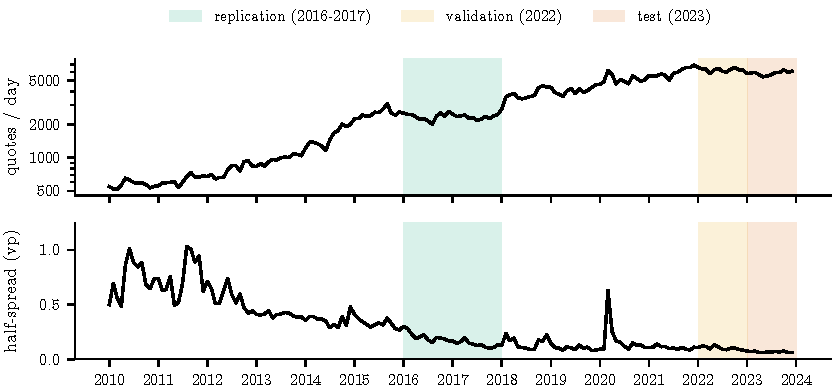
\includegraphics[width=\linewidth]{data.pdf}
  \caption{SPX chains after cleaning: monthly medians of quotes per day (log scale) and of the
  half-spread in implied vol (vol points, vp). Shading marks the evaluation windows; each conditional
  model trains only on days before the window it is scored on (\cref{tab:windows}).}
  \label{fig:data}
\end{figure}

\subsection{Synthetic panels}

Synthetic panels have a known arbitrage-free truth and labelled mispricings. Each business day
draws a variance state from a log-variance Ornstein--Uhlenbeck process correlated with spot, and
quotes Heston prices~\citep{heston1993}, computed with the COS method~\citep{fang2008}, with the
day's state as initial variance, on a realistic listing of weekly and monthly expiries. Quotes get
bid-ask spreads, noise inside the spread and tick rounding. Mispricings are injected as isolated
strikes or segments of 3--6 neighbouring strikes, shifted by 2--5 half-spreads; they persist and
decay by half each day, so a perfect detector's flags revert by $-0.50$, $-0.875$ and $-0.97$ of
their size at 1, 3 and 5 days. The main panel covers 2020--2022 (training, validation and test
year); a second panel from the same generator with a new seed (2012--2019) adds training days, and
a third (2023, a further seed) was generated for the final test and not inspected beforehand.

\subsection{Windows and protocol}

\Cref{tab:windows} lists the roles of the windows. The project was built on SPX 2018--2023;
2010--2017 was added later, for a longer training history and a second test window that no choice
was tuned on. Every setting that the test runs use was chosen on SPX 2022 or Heston 2021 and
committed before the test run.

\begin{table}[t]
  \centering\small
  \caption{Evaluation windows. A ``run'' is one evaluation of frozen settings on a test window; each
  later run was motivated by a finding and frozen on the validation years first.}
  \label{tab:windows}
  \begin{tabular}{@{}lp{5.6cm}p{6.6cm}@{}}
    \toprule
    window & role & runs on it \\
    \midrule
    SPX 2010--2021 & training of the conditional model (first 2018--2021) & -- \\
    SPX 2022 & validation: every model, penalty, detector and backtest setting & -- \\
    SPX 2023 & test & 4: mispricing tests; walk-forward refits and follow-up detectors; full-history model; mispricing tests on refitted surfaces \\
    SPX 2016--2017 & replication (conditional model retrained on 2010--2015) & 2: every model and detector; refits \\
    Heston 2020 / 2021 & training / validation & -- \\
    Heston 2022 & test & 3: detectors; follow-up detectors; refits \\
    Heston 2023 (fresh seed) & test of the nine-year conditional model & 2: follow-up detectors; refits \\
    \bottomrule
  \end{tabular}
\end{table}

Surface models are compared on blocks of two consecutive trading days every ten days (52 days of
SPX 2022, 50 of 2023 and 101 of 2016--2017). Days with heavy model-free arbitrage or poor forward
coverage are screened out. In each expiry the outer 10\% of strikes on each side are held out to
measure wing extrapolation and a random 15\% of interior strikes to measure interpolation, with the
split seeded by the date so that every model sees the same one. We report the IV RMSE in vol points
(vp) on fitted and held-out quotes, the share of model IVs inside the quoted bid-ask, and the share
of a dense $(k,T)$ grid on which the calendar or butterfly condition fails, over the quoted domain
widened by 50\% on each side. Synthetic panels also report the error against the true surface. The
mispricing tests (\cref{sec:mispricing}) use every trading day of their windows.
